\documentclass[11pt,1in]{article}
%\documentclass{amsart}
\usepackage{amsmath, amssymb,amsfonts}
\usepackage{physics}
\usepackage[margin=1in]{geometry}
\usepackage{cite}
\usepackage{booktabs}
\usepackage{graphicx}
\usepackage{epstopdf}
\usepackage{float}
\usepackage{siunitx}
\usepackage[numbered,framed]{matlab-prettifier}
\newtheorem{definition}{Definition}

\newenvironment{Example}[2][Example]{\begin{trivlist}
		\item[\hskip \labelsep {\bfseries #1}\hskip \labelsep {\bfseries #2.}]}{\end{trivlist}}
\usepackage{hyperref}


\lstset{
	caption			   = {MATLAB Source Code},
	style              = Matlab-editor,
	basicstyle         = \tiny\mlttfamily,
	escapechar         = ",
	mlshowsectionrules = true,
	label			   = {lst:source_code}
}

\title{Analyzing Non-linear Ordinary Differential Equations\\ {\small MATH 26600}}
\author{Rutuj Gavankar}
\date{}

\begin{document}

\maketitle

\section{Introduction}
A Differential Equation is an equation describing the relationship of a function and its derivatives. Differential equations can be used to model physical phenomena and predict how a system changes. Ordinary differential equations (ODE's) are differential equations involving only one independent variable. A linear differential equation is one where every term of the dependent  variable is linear. The most general form of an $n$'th order linear differential equation is 
\begin{align}
\sum_{i = 0}^{n} a_i(t) \frac{\dd[(i)]{y(t)}}{\dd{t^{(i)}}} &= b(t) \label{eq:linear}
\end{align}
where $y(t)$ is the dependent variable and $t$ is the independent variable. Since the derivative is a linear operator, every term in Eq. \ref{eq:linear} is linear in $y$. An $n$'th order linear ODE can be reduced to a system of $n$ equations by introducing substitution $y_{i+1}(t) = \frac{\dd[(i)]{y(t)}}{\dd{t^{(i)}}}$. Thus the system can be written in vector-matrix notation as 
\begin{align}
\derivative{}{t} \begin{bmatrix}
y_1 \\ \vdots  \\\ y_n 
\end{bmatrix}  &= 
\begin{bmatrix}
a_{11} & \ldots & a_{1n} \\
\vdots & \ddots & \vdots \\
a_{n1} & \ldots & a_{nn}
\end{bmatrix}
\begin{bmatrix}
y_1 \\ \vdots  \\\ y_n \label{eq:matrix_notation}
\end{bmatrix}
\end{align}
which can be equivalently written as $\vec{Y}'(t) = A \vec{Y}$. The system in Eq. \ref{eq:matrix_notation} has thus been reduced to an eigenvalue problem with the general solution with is analytical and of the form 
\begin{align}
\vec{Y}(t) &= \begin{bmatrix}
c_1 e^{\lambda_1 t} \\ \vdots  \\\ c_n e^{\lambda_n t}  \label{eq:general_sol}
\end{bmatrix}
\end{align}
where $\lambda$ are the eigenvalues of the matrix $A$. 
\subsection{Linearizing a system}
A system of linear differential equations is easy to analyze and has analytical solutions in most cases. To analyze as system of non-linear equations, the system must be linearized. 
Let 
\begin{align}
\derivative{x}{t} &= F(x, y) \\
\derivative{y}{t} &= G(x , y)
\end{align}
be a system of first-order differential equations. The steady-state solutions of this system are the solutions for which  $x(t)$ and $y(t)$ are invariant. That is to say,
\begin{align}
    F(x,y) &= 0 \\
    G(x,y) &= 0
\end{align}
We can analyzing this system around these equilibrium points by making linear approximations of the function around these points. Using first order Taylor series expansion for $F$ and $G$ we get
\begin{align}
    F(x,y) &\approx F(x_0, y_0) + F_x(x_0, y_0)(x - x_0) + F_y(x_0, y_0)(y - y_0) \\
    G(x,y) &\approx G(x_0, y_0) + G_x(x_0, y_0)(x - x_0) + G_y(x_0, y_0)(y - y_0)
\end{align}
where $x_0$ and $y_0$ are the equilibrium points for the system. The system can be re-written in matrix-vector notation as 
\begin{align}
    \begin{bmatrix}
    \derivative{x}{t} \\
    \derivative{y}{t}
    \end{bmatrix} &= 
    \begin{bmatrix}
    F_x(x_0, y_0) & F_y(x_0, y_0)\\
    G_x(x_0, y_0) & G_y(x_0, y_0)
    \end{bmatrix}
    \begin{bmatrix}
    x - x_0 \\
    y - y_0
    \end{bmatrix}
\end{align}Now, let $x - x_0$ be $u$ and $y - y_0$ be $v$, and $\Vec{v}$ be the vector $\left<u ,v\right>$
\begin{align}
    \therefore \derivative{\Vec{v}}{t} &= J\Vec{v} \label{eq:vec_mat}
\end{align}
Where $J$ is the Jacobian matrix, $$J = \begin{bmatrix}
    F_x(x_0, y_0) & F_y(x_0, y_0)\\
    G_x(x_0, y_0) & G_y(x_0, y_0)
    \end{bmatrix}$$
Now, Eq. \ref{eq:vec_mat} is an eigenvalue problem. The local stability and the behaviour of the system around the equilibrium points can be inferred from the eigenvalues of $J$. 

\subsection{Characterizing a system}
Near the equilibrium points, the non-linear system has similar behavior to the linear approximation, and thus, the stability of the system can be analyzed by analyzing the eigenvalues of the system. Let $\lambda_{1,2}$ be the eigenvalues of the system.
\begin{enumerate}
	\item If the eigenvalues of the system are real and positive at an equilibrium point, ($\lambda_{1,2} > 0$), the point is a \emph{nodal-source}. The solutions tend to diverge away from this point. The system is unstable around this point. 
	\item If the eigenvalues of the system are real and negative at an equilibrium point, ($\lambda_{1,2} < 0$),the point is a \emph{nodal-sink}. The solutions tend to converge towards this point. The system is stable around this point. 
	\item If the eigenvalues of the system are real, but $\lambda_1 < 0$ and $\lambda_2 > 0$, the point is a \emph{saddle point}. The solutions tend to diverge away from this point. The system is unstable around this point.
	\item If the eigenvalues of the system imaginary, $(\lambda_{1,2} = \pm k i)$, the point is a \emph{center}.  The solutions tend to oscillate around this point. The system is stable around this point.
	\item If the eigenvalues of the system are complex, $(\lambda_{1,2} = a \pm b i)$, and $\Re{\lambda_{1,2}}> 0$, the point is a \emph{spiral-source}. The solutions tend to spiral-out from the equilibrium point. The system is unstable around this point.
	\item If the eigenvalues of the system are complex, $(\lambda_{1,2} = a \pm b i)$, and $\Re{\lambda_{1,2}}< 0$, the point is a \emph{spiral-source}. The solutions tend to spiral-in to the equilibrium point. The system is stable around this point.
\end{enumerate}

\subsection{Quantitative Analysis of a System}
To graphically analyze a system of differential equations and get a quantitative understanding of what is happening to the system as time evolves, the nullclines can be plotted on the phase plane. 
\begin{definition}[Nullclines \cite{diff_eq}]
	For a system 
	\begin{align*}
	\derivative{x}{t} &= f(x,y) \\
	\derivative{y}{t} &= g(x,y)
	\end{align*}
	the x-nullcline is the set of points $(x,y)$ where $f(x,y) = 0$ and y-nullcline is the set of points where $g(x,y) = 0$ 
\end{definition}


That is, $x$-nullcline are a set of points with vertical slope and $y$-nullcline are a set of points with horizontal slope. The intersection of the $x$ and $y$ nullclines is the set of points where both, the horizontal and vertical components of the slope are zero. That is, the system is not changing with respect to time at those points. Therefore, the intersection of the $x$ and $y$ nullclines gives the steady-state points of the system. By looking at the direction of the vector field around the steady-state points, the stability of the points can be determined. That is, if the vectors around the steady-state points are \emph{diverging} from it, the point is a \emph{source}. If the vectors are \emph{converging} towards it, the point is a \emph{sink}.  
\subsection{Examples and Solutions}
\begin{Example}{1} \cite[p.~488]{diff_eq}
	Consider the system for $(x,y \geq 0)$
	\begin{align*}
    \derivative{x}{t} &= x(10 - x - y) \\
    \derivative{y}{t} &= y(30 - 2x - y)
\end{align*}
The Jacobian of the system is 
\begin{align*}
    J = \begin{bmatrix}
    10 - 2x - y & -x \\
    -2y & 30 - 2x - 2y
    \end{bmatrix}
\end{align*}
The system has equilibrium points at $(0,0)$, $(10,0)$, $(0,30)$. Analyzing the system at $(0,0)$,
\begin{align*}
    J|_{(0,0)} &= \begin{bmatrix}
    10 & 0 \\
    0 & 30
    \end{bmatrix}
\end{align*}
Since $J$ is a diagonal matrix, the eigenvalues of $J$ are the elements along its diagonal. That is, $\lambda_{1,2} = \{ 10, 30 \}$. Since both the eigenvalues are real and positive, the point $(0,0)$ is a nodal-source.
Similarly, analyzing the system at $(10,0)$,
\begin{align*}
    J|_{(10,0)} &= 
    \begin{bmatrix}
    -10 & -10\\
    0 & 10 
    \end{bmatrix}
\end{align*}
The eigenvalues of $J$ are $\lambda_{1,2} = \{-10, 10\}$. Since both the eigenvalues are real and nonzero, and $\lambda_1 < 0$, $\lambda_2 > 0$, the point $(10,0)$ is a saddle point. 
Now analyzing the system at $(0,30)$,
\begin{align*}
J|_{(0,30)} &= \begin{bmatrix}
-20 & 0 \\
-60 & -30 
\end{bmatrix}
\end{align*}
The eigenvalues for $J$ are $\lambda_{1,2} = \{-30, -20\}$. Since both eigenvalues are real and negative, $(0,30)$ is a nodal-sink. 
Now to graphically analyze the system, the nullclines can be plotted in the phase plane.
To find the $x$-nullclines,
\begin{align*}
\derivative{x}{t} &= 0\\
\therefore x(10 - x -y) &= 0
\end{align*}
That is, $x = 0$ or $y = 10 - x$. 
To find the $y$-nullclines,
\begin{align*}
\derivative{y}{t} &= 0\\
\therefore y(30 - 2x - y) &= 0
\end{align*}
That is, $y = 0$ or $y = 30 - 2x$. 
The nullclines intersect at $(0,0)$, $(10,0)$, $(15,0)$, $(0,30)$, which are the steady-state points of this system. In Fig.\ref{fig:example1} the quantitative analysis of the system can be graphically verified by observing the direction of the vector fields around steady-states. 
The 
\begin{figure}[H]
	\centering
	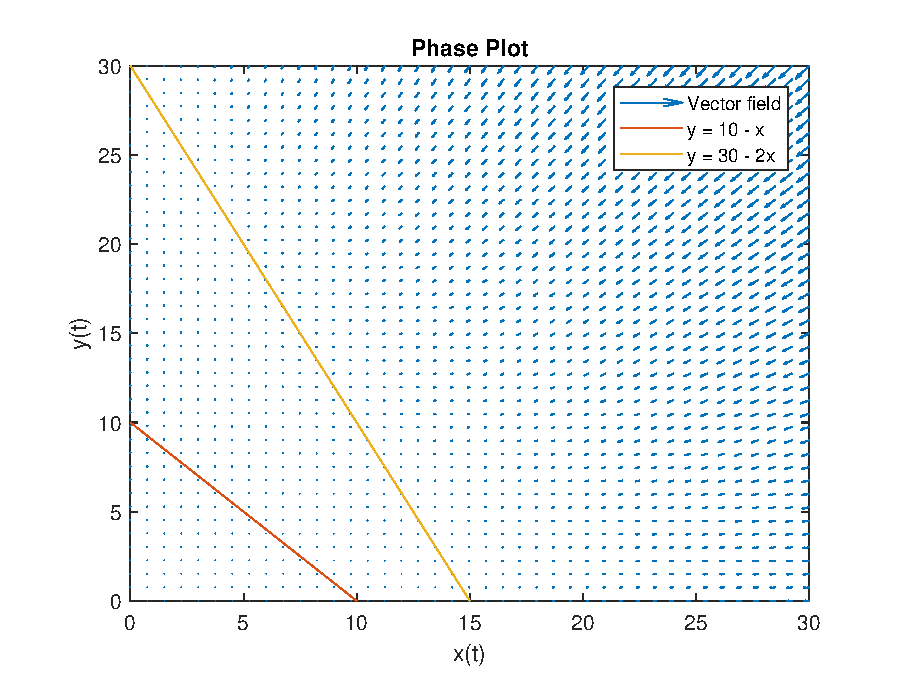
\includegraphics[width=\linewidth,height=.85\linewidth]{Figures/example_1}
	\caption{Nullclines and vector fields}
	\label{fig:example1}
\end{figure}

\end{Example}

\begin{Example}{2}
	\cite[p.~488]{diff_eq}
	Consider the system for $(x,y \geq 0)$
	\begin{align*}
	\derivative{x}{t} &= x(2 - x - y)\\
	\derivative{y}{t} &= y(y - x^2)
	\end{align*}
	The Jacobian of the system is
	\begin{align*}
	J = \begin{bmatrix}
	2 -2x  -y & -x \\
	-2xy & 2y - x^2 
	\end{bmatrix}
	\end{align*}
	Steady-states in the region $(x,y \geq 0)$ are $(0,0)$ , $(1,1)$, and $(2,0)$. Analyzing point $(0,0)$,
	\begin{align*}
	J|_{(0,0)} = \begin{bmatrix}
	2 & 0 \\
	0 & 0
	\end{bmatrix}
	\end{align*}
	The eigenvalues of $J$ are $\lambda_{1,2} = \{2, 0\}$. Since the eigenvalues are non-negative, the solution diverges from $(0,0)$ and the system is unstable around this point. 
	At $(1,1)$
	\begin{align*}
	J|_{(1,1)} &= \begin{bmatrix}
	-1 & -1 \\
	-2 & 1
	\end{bmatrix}
	\end{align*}
	The eigenvalues of $J$ at this point are $\lambda_{1,2} = \pm \sqrt{3}$. Since both the eigenvalues have opposite signs, the point $(1,1)$ is a saddle point, and the system is unstable around this point. At point $(2,0)$,
	\begin{align*} J|_{(2,0)} &=
	\begin{bmatrix}
	-2 & -2 \\
	0 & - 4
	\end{bmatrix}
	\end{align*} 
	The eigenvalues of $J$ at this point are $\lambda_{1,2} = \{-2,-4\}$. Since both the eigenvalues are negative, the point $(2,0)$ is a nodal-sink, and the system is stable around this point. The $x$-nullclines are given by 
	\begin{align*}
	\derivative{x}{t} &= 0 \\
	\therefore x(2 - x - y) &= 0
	\end{align*}
	That is, $x = 0$ and $y = 2 - x$. The $y$-nullclines are given by 
	\begin{align*}
	\derivative{y}{t} &= 0\\
	\therefore y(y - x^2 ) &= 0
	\end{align*}
	That is, $y = 0$ and $y = x^2$. The $x$ and $y$ nullclines intersect at $(0,0)$, $(1,1)$ and $(2,0)$, which are the steady-states of the system for $(x,y \ge 0)$. Figure \ref{fig:example2} shows the vector field and $xy$ nullclines on the phase plane. 
\begin{figure}[H]
	\centering
	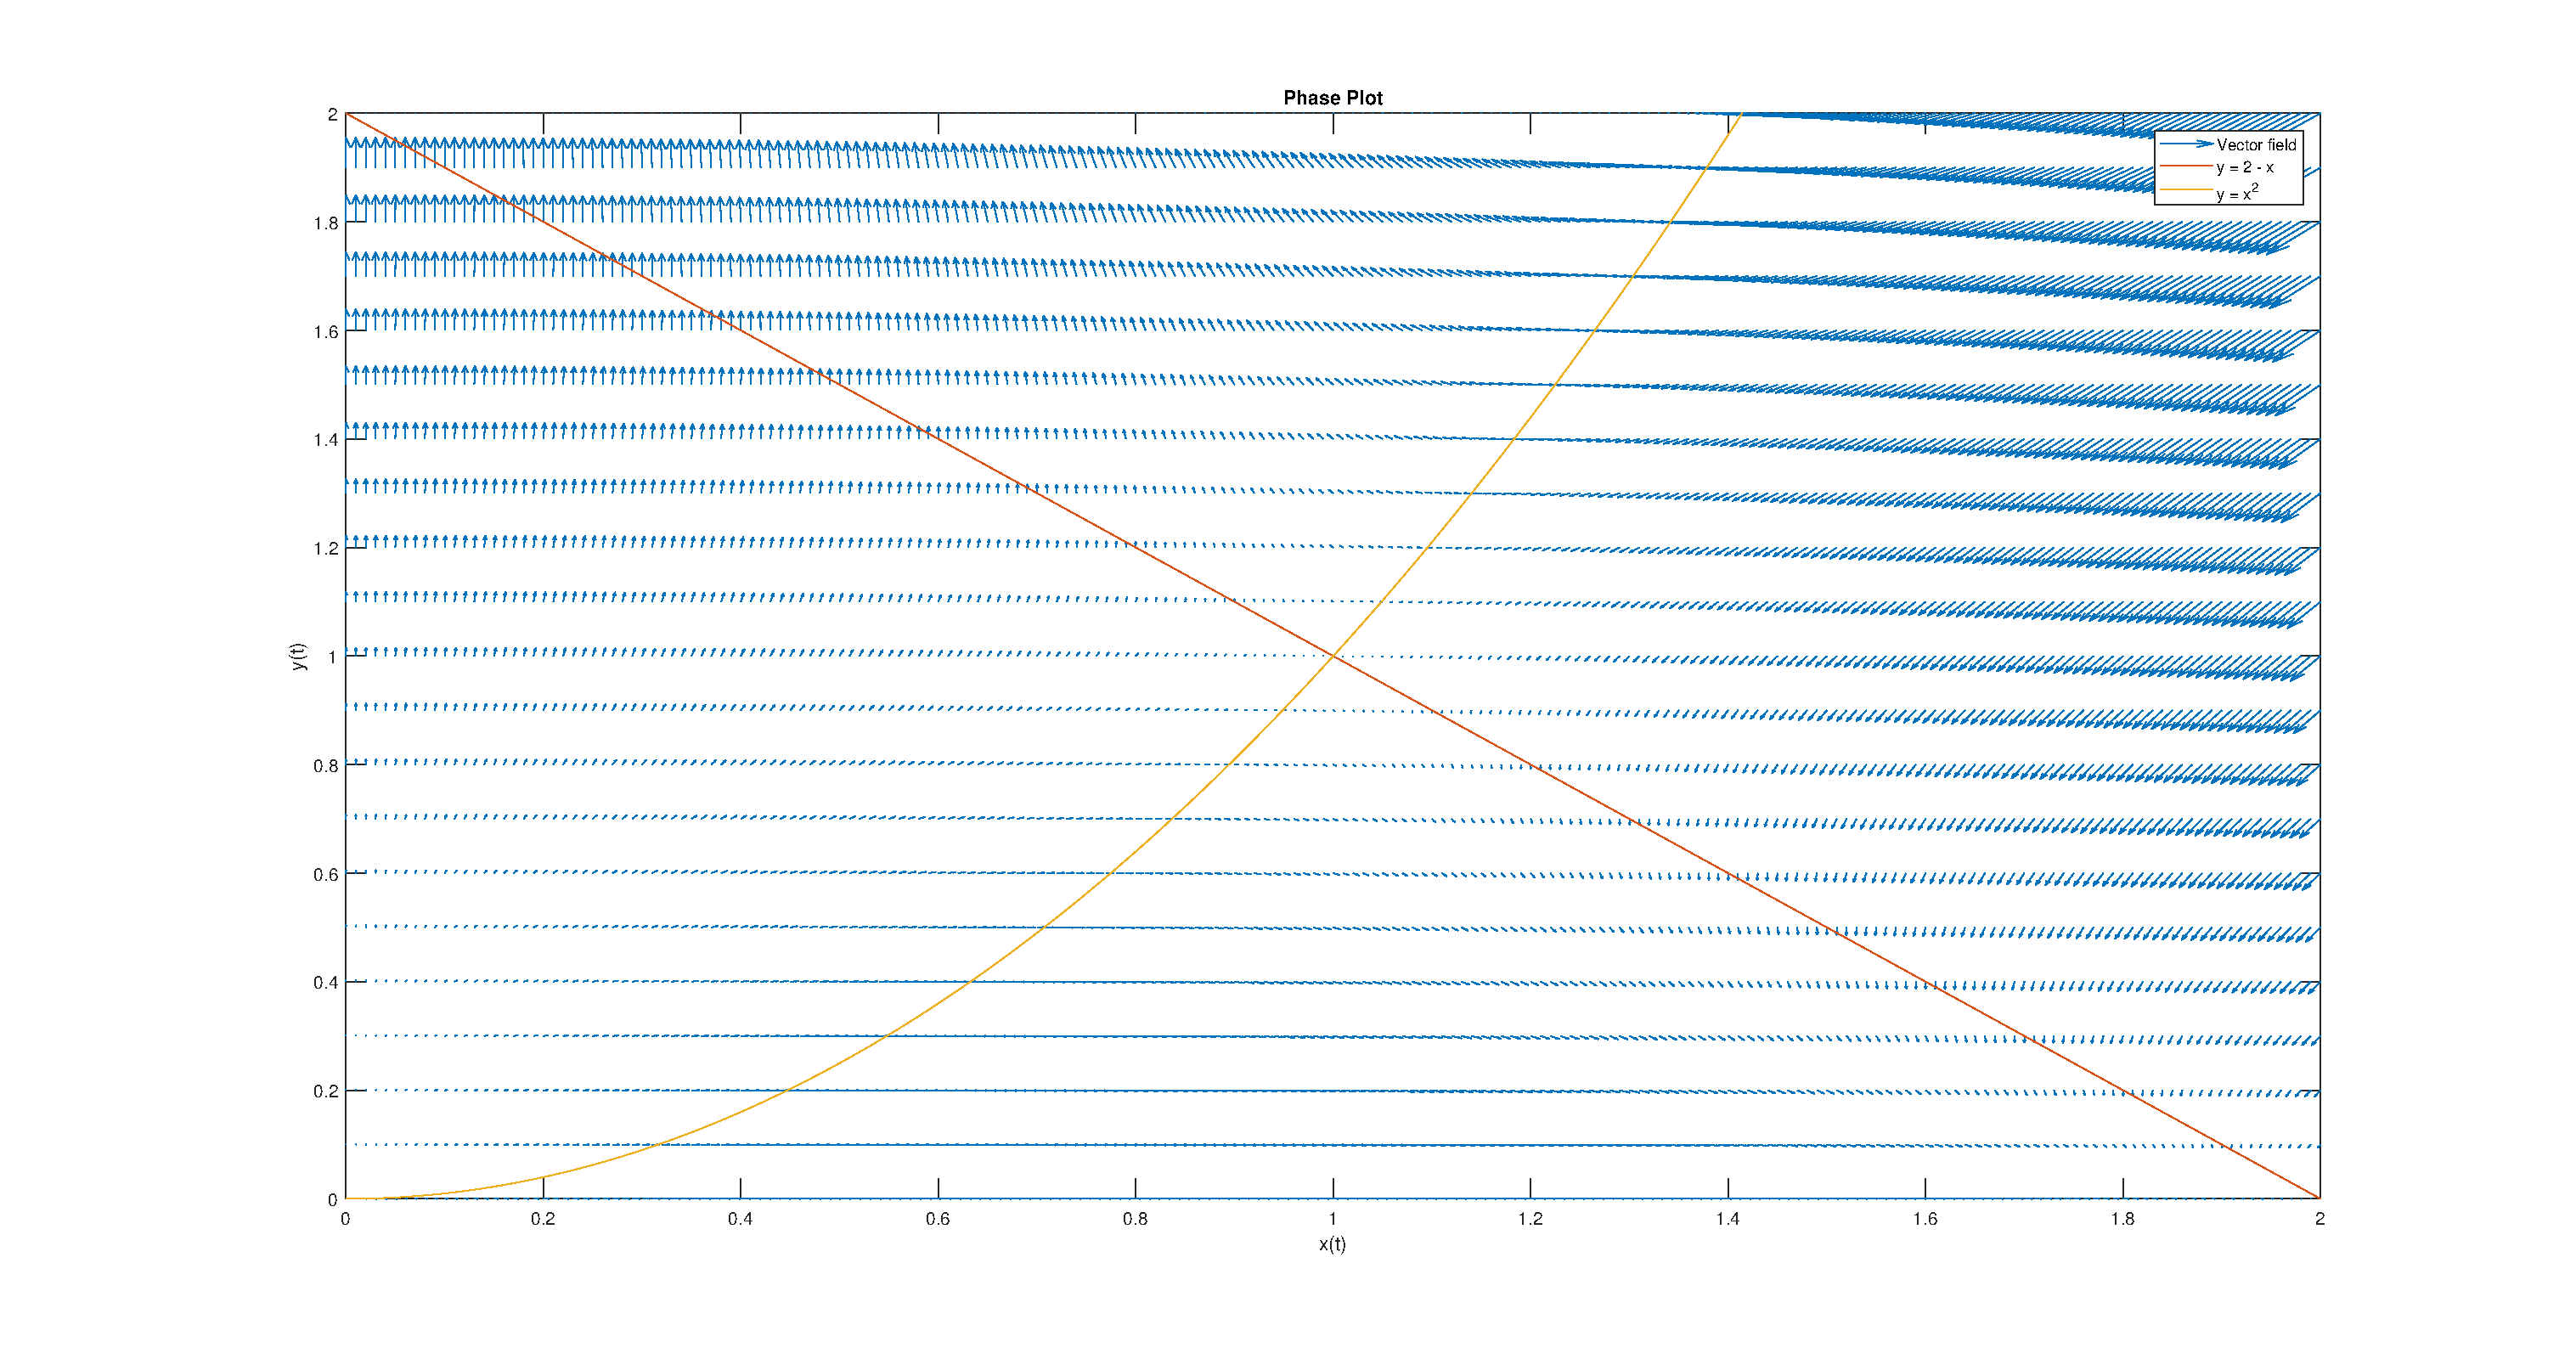
\includegraphics[trim={2in 0 2in 0},width=\linewidth]{Figures/example_2}
	\caption{Nullclines and vector fields}
	\label{fig:example2}
\end{figure}
\end{Example}
\begin{Example}{3}
	\cite[p.~487]{diff_eq}
	\begin{align*}
	\derivative{x}{t} &= x(x - 1)\\
	\derivative{y}{t} &= x^2 - y
	\end{align*}
	For 
	\begin{enumerate}
		\item $x_0 = -1$, $y_0 = 0$
		\item $x_0 = 0.8$, $y_0 = 0$
		\item $x_0 = 1$, $y_0 = 3$
	\end{enumerate}
\begin{figure}[H]
	\centering
	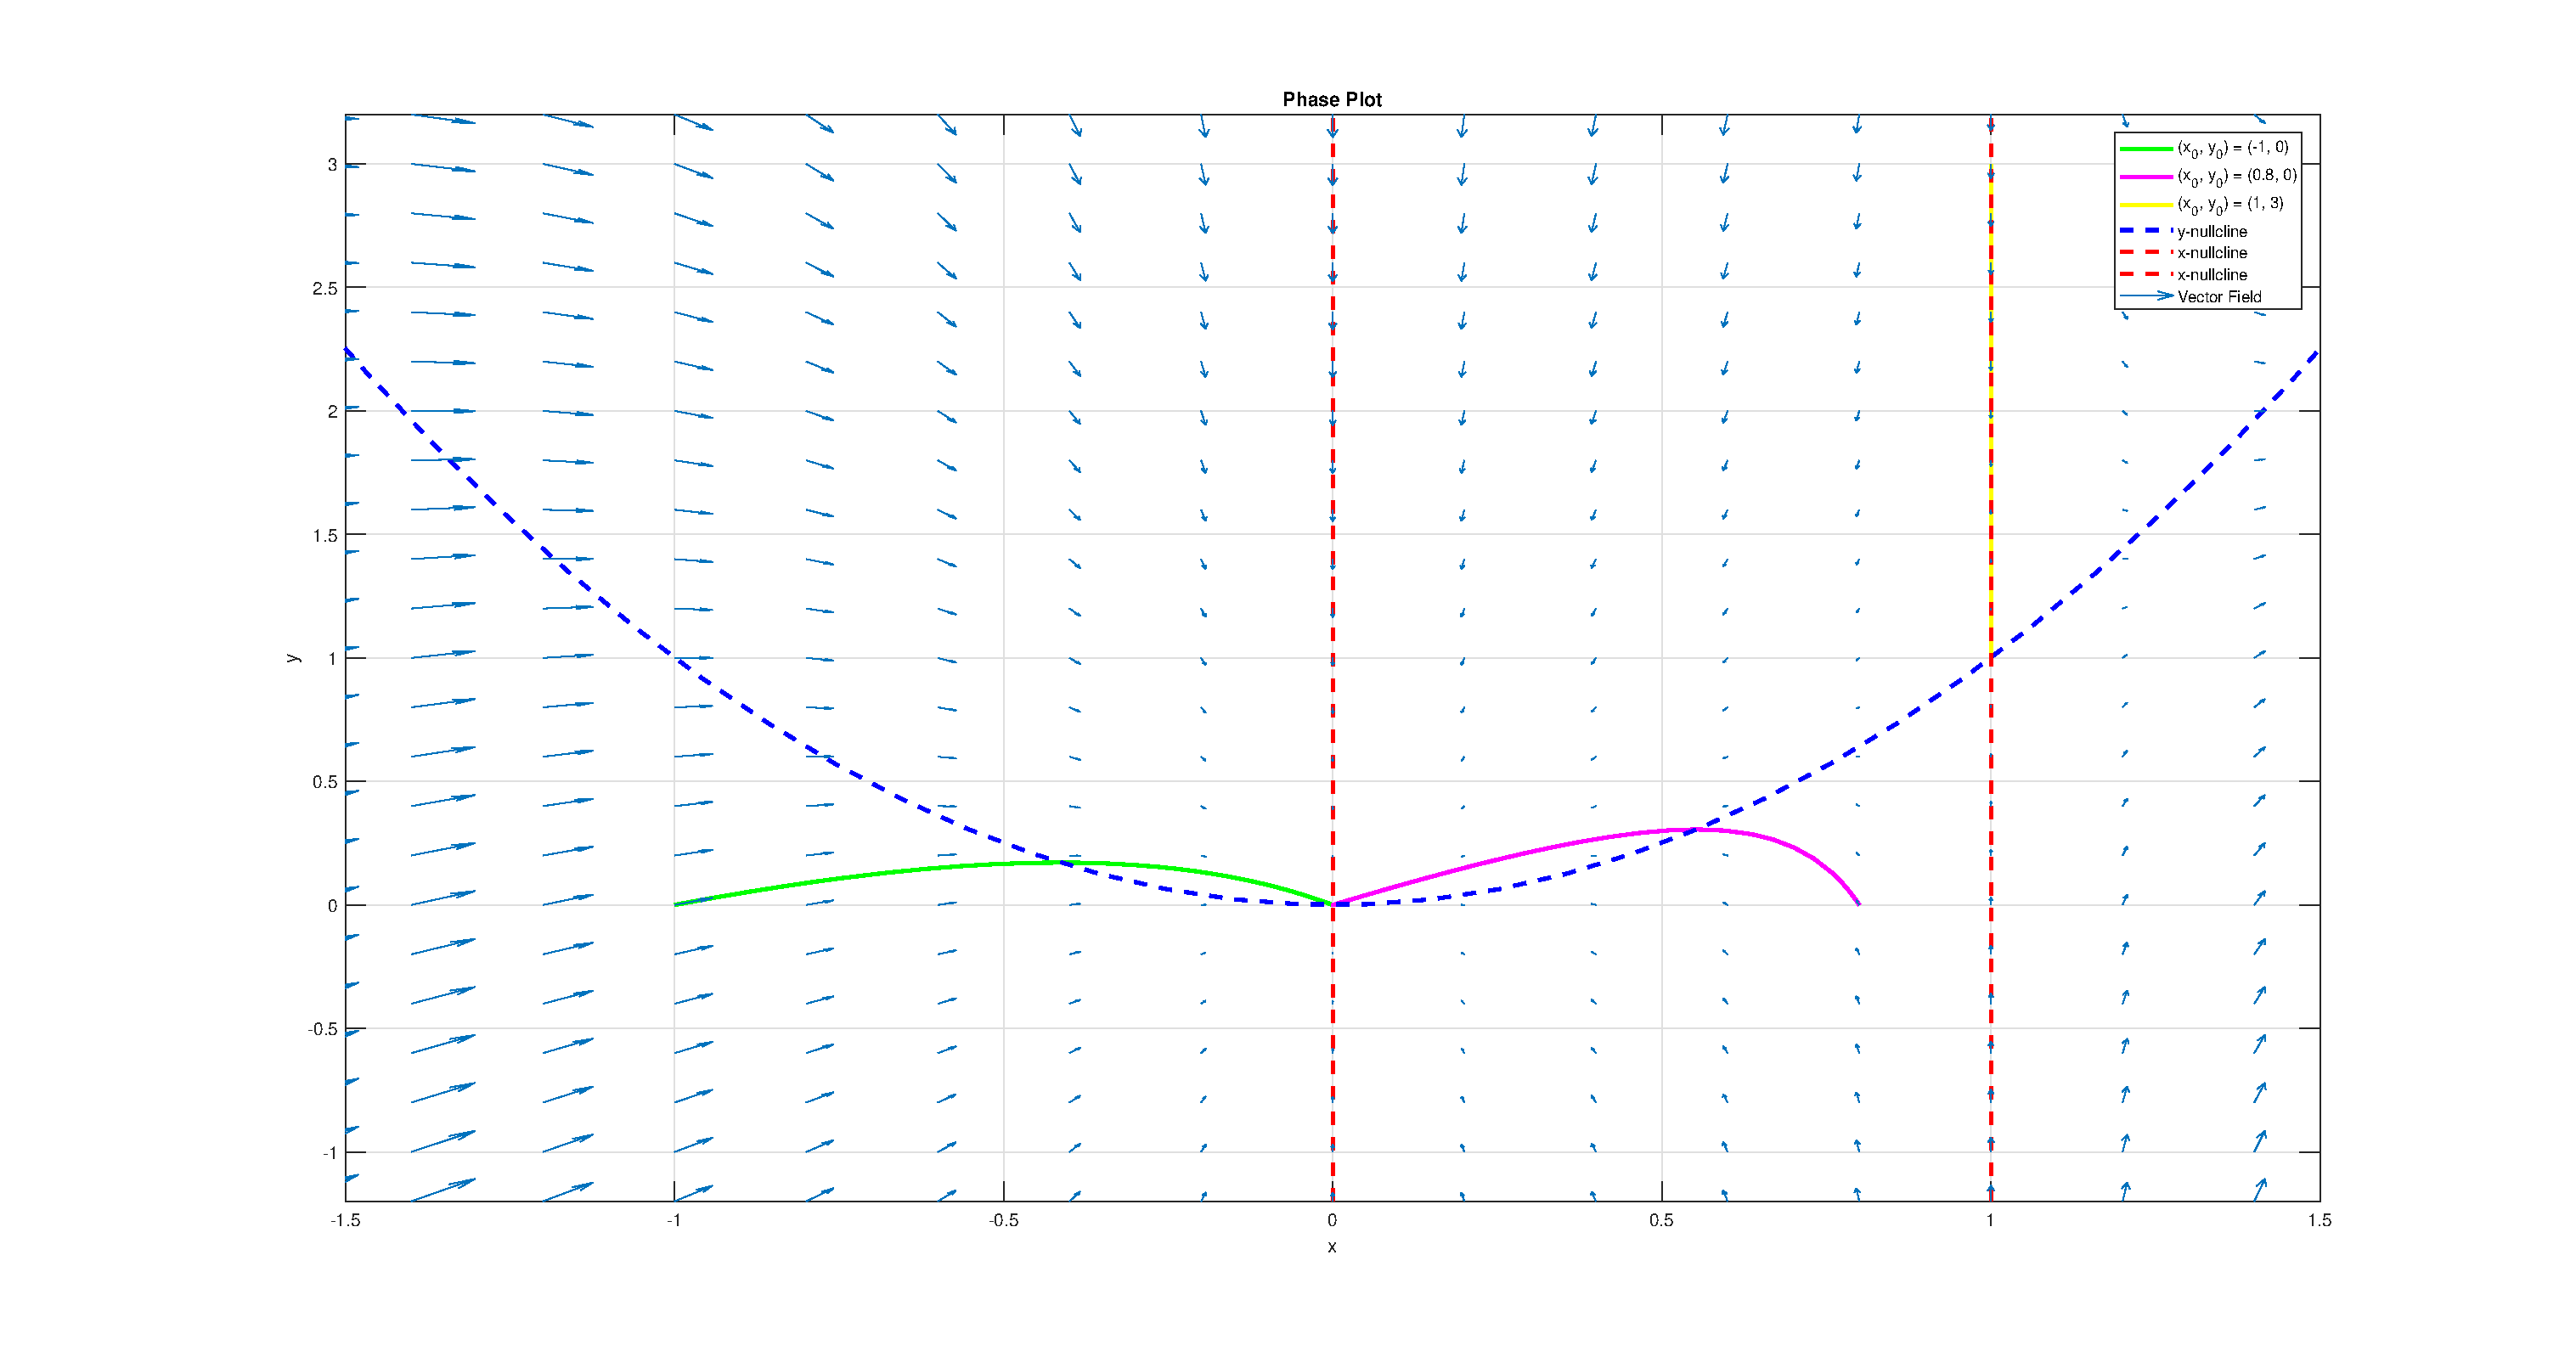
\includegraphics[trim={2in 0 2in 0},width=1\linewidth]{Figures/example_3_phase}
	\caption{Solution Curves and Nullclines}
	\label{fig:example3}
\end{figure}
Figure \ref{fig:example3} shows the solution curves in the $xy$-plane with $t$ as an implicit parameter. The direction of the arrows shows the tendancy of the solutions as $t\rightarrow\infty$. The above system has $x$-nullclines at $x = 0$ and $x = 1$ and $y$-nullclines at $y = x^2$. The interesection points of the nullclines are the steady-states of the system. The MATLAB source code for the generated plots can be found in Listing \ref{lst:source_code}.
 
\end{Example}
\section{Hamiltonian Systems}
\subsection{Conserved Quantities and Hamiltonians}
\begin{definition}[Conserved quantity \cite{diff_eq}]
A real-valued function $H(x,y)$ of the two variables $x$ and $y$ is a conserved quantity for a system of differential equations if it is constant along all solution curves of the system. 
\begin{align}
\derivative{}{t}H(x(t), y(t) = 0
\end{align}
\end{definition}
\newpage
\begin{definition}[Hamiltonian system \cite{diff_eq}]
A system of differential equations is called a \textit{Hamiltonian system} if there exists a real-valued function $H(x,y)$ such that 
\begin{align}
\derivative{x}{t} &= \frac{\partial H}{\partial y} \label{ham_1} \\
\derivative{y}{t} &= - \frac{\partial H}{\partial x} \label{ham_2}
\end{align}
\end{definition}
All Hamiltonian functions are conserved quantities.
\subsection{Characterizing a Hamiltonian system}
The Jacobian of such a system is given by 
\begin{align}
J &= \begin{bmatrix}
\frac{\partial^2H}{\partial x \partial y} & \frac{\partial^2H}{\partial y^2} \\
\frac{\partial^2H}{\partial x^2} & -\frac{\partial^2H}{\partial x \partial y}
\end{bmatrix} \\
&= \begin{bmatrix}
\alpha & \beta \\
\gamma & -\alpha
\end{bmatrix}
\end{align}
The eigenvalues of the matrix $J$ are $\lambda_{1,2} = \pm \sqrt{\alpha^2 + \beta\lambda}$. Now,
\begin{enumerate}
	\item If $\alpha^2 + \beta\lambda > 0$, both eigenvalues will be real and have opposite signs, and equilibrium point will be a saddle. 
	\item If $\alpha^2 + \beta\lambda < 0$, both eigenvalues are imaginary and complex-conjugates. The equilibrium  point will be a center. 
	\item If $\alpha^2 + \beta\lambda = 0$, the only eigenvalue is $\lambda = 0$. This test is inconclusive and requires further analysis, but since the system is Hamiltonian, the equilibrium point cannot be a source or a sink \cite{diff_eq}.  
\end{enumerate}
\subsection{Constructing the Hamiltonian function \label{sec:constructing_hamiltonian}}
If a system 
\begin{align}
x'(t) &= f(x,y) \\
y'(t) &= g(x,y)
\end{align}
is Hamiltonian, with an unknown Hamiltonian function $H(x,y)$ then, \cite[pp. 499]{diff_eq}
\begin{align}
\frac{\partial f}{\partial x} &= -\frac{\partial g}{\partial y}  \\
f(x,y) &= \frac{\partial H}{\partial y} \\
g(x,y) &=  - \frac{\partial H}{\partial x}
\end{align}
That is,
\begin{align}
H(x,y) &= \int f(x,y) \dd{y} + \phi(x)
\end{align}
where $\phi(x)$ is a scalar function that is independent of $y$. That is,
\begin{align}
\phi'(x) = - g ( x , y ) - \frac { \partial } { \partial x } \int f ( x , y ) \dd{y}
\end{align}
Thus the Hamiltonian function can be constructed by 
\begin{align}
H(x,y) &= \int f(x,y) \dd{y} + \int \phi'(x) \dd{x}
\end{align}
\subsection{Applications of Hamiltonian Systems - Non-linear Pendulum}
For an ideal-pendulum with mass $m = 1$, length $l = 1$ and no friction, the system describing the motion in polar coordinates is 
\begin{align}
\derivative{\theta}{t} &= \omega \\
\derivative{\omega}{t} &= -g \sin\theta
\end{align}  
where $\theta$ is the angular displacement and $\omega$ is the angular velocity of the pendulum. 

The system has periodic steady-states at $(\theta, \omega ) = (\pm n\pi , 0)$ where $n = 0,1,2,\ldots$. Physically, since there is no friction in the system, the total energy has to be conserved at every point in the system, implying that the total energy of the system is the Hamiltonian function for the system. The total energy for the system at any point in space and time is the total kinetic energy $T$ and the total potential energy $U$. The Hamiltonian can be constructed by $H(\theta, \omega, t) = T(\omega, t) + U(\theta, t)$ \cite{engr_math}. That is,
\begin{align}
H(\theta,\omega, t) &= \frac{m l^2 \omega^2}{2} + mgl(1 - \cos\theta) \\
&= \frac{\omega^2}{2} - g\cos\theta \label{eq:hamiltonian_pendulum}
\end{align}
since $m,l = 1$ and $g$ is a constant. Alternatively, the Hamiltonian can be formulated by the method in Section \ref{sec:constructing_hamiltonian}. 

As seen in Figure \ref{fig:pendulum_phase} and Figure \ref{fig:pendulum_solution_curves}, the solution curves depend on the initial conditions. 
\begin{enumerate}
	\item If the initial angle $\theta$ is $n\pi$ and the initial velocity $\omega$ is $0$, that is, parallel to the vertical axis and at rest, the pendulum is in equilibrium and does not more. 
	\item If the initial angle $\theta < 2n\pi$ and initial velocity $\omega = 0$, the pendulum never crosses $(2n + 1)\pi$, and thus always oscillates back and forth. This case is similar to the linear pendulum approximation (Fig. \ref{fig:pendulum_phase}, curve A). 
	\item If the pendulum starts off with an initial velocity that is greater than a critical velocity $\omega_0$, the pendulum rotates forever with a non-zero velocity at all times (Fig. \ref{fig:pendulum_phase}, curve B).
\end{enumerate}

\begin{figure}[H]
	\centering
	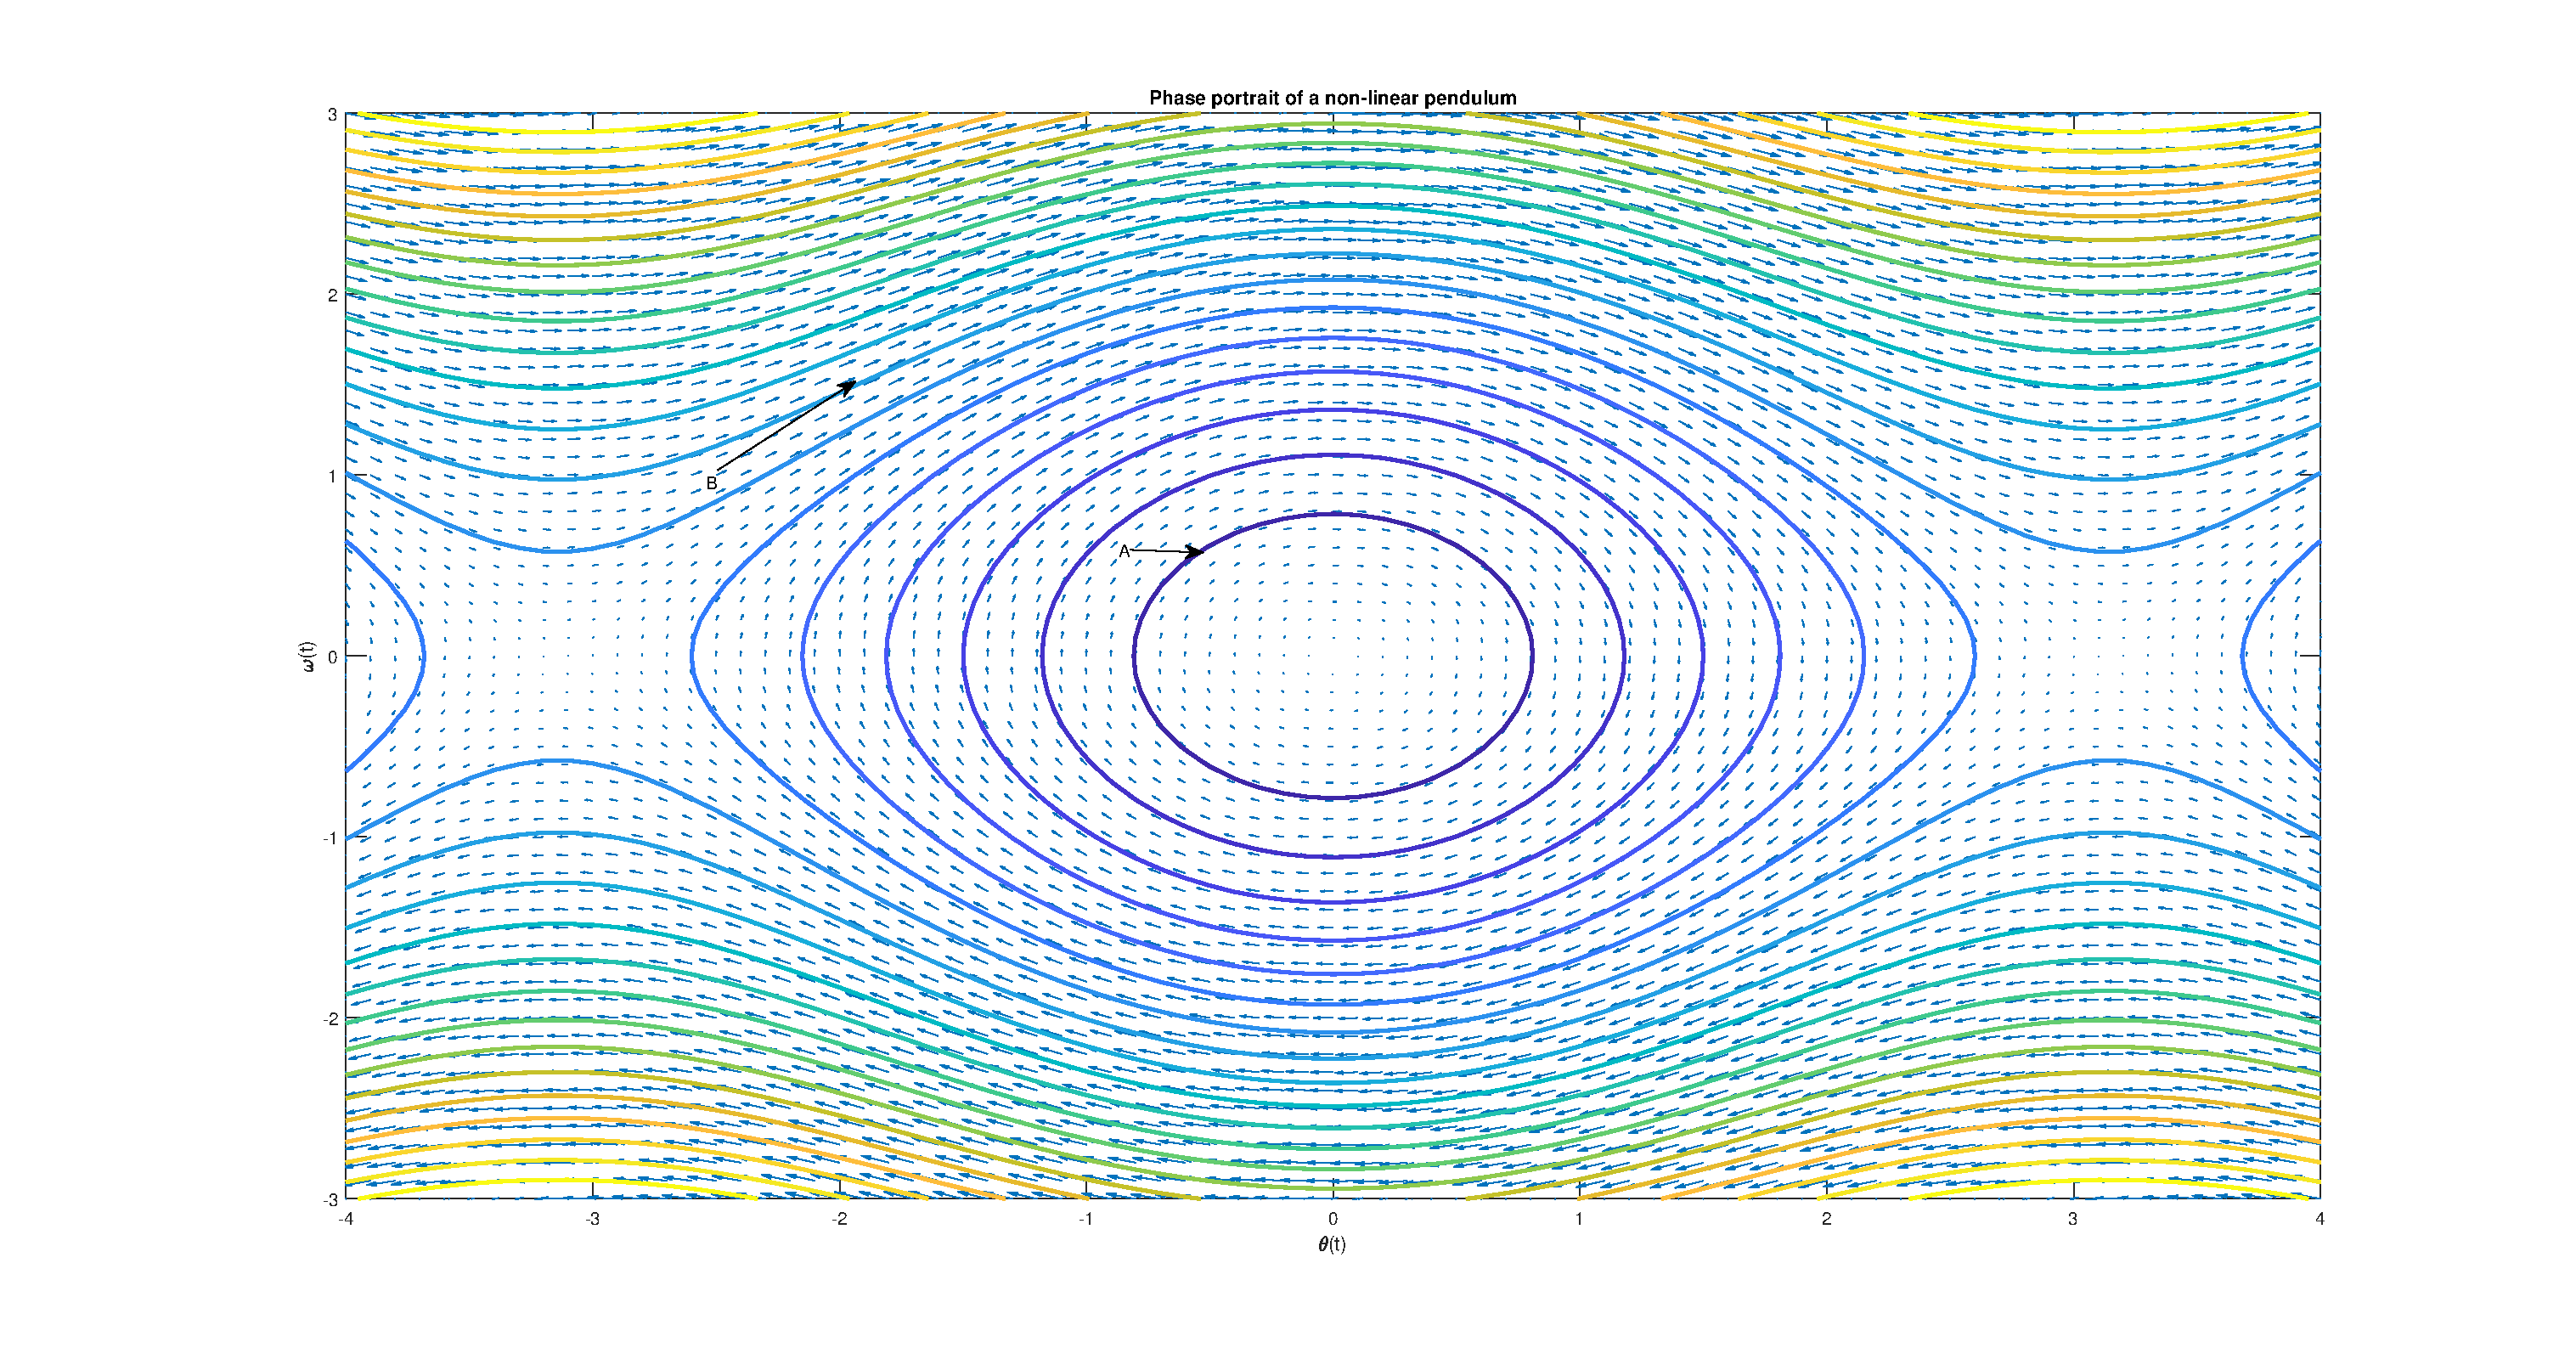
\includegraphics[trim={2in 0 1.5in 0}, width=\linewidth]{Figures/pendulum_phase}
	\caption{Phase portrait of a non-linear pendulum}
	\label{fig:pendulum_phase}
\end{figure}


\subsection{Examples}
\begin{Example}{1}
	\begin{align*}
	\derivative{x}{t} &= y \\
	\derivative{y}{t} &= x^2 - a
	\end{align*}
	where $a$ is a parameter. \\
	{\bfseries Solution\\}
	\begin{align*}
	H(x,y) &= \frac{y^2}{2} - \frac{x^3}{3} + ax
	\end{align*}
	To verify that this system is a Hamiltonian system if $H$ is the Hamiltonian function,
	\begin{align*}
	\frac{\partial}{\partial y}H(x,y) &= y\\
	&= \derivative{x}{t}
	\end{align*}
	and,
	\begin{align*}
	- \frac{\partial}{\partial x} H(x,y) &= x^2 - a\\
	&= \derivative{y}{t}
	\end{align*}
	Since $H_x(x,y) = - y'(t)$ and $H_y(x,y) = x'(t)$, the system is Hamiltonian for $H(x,y)$ as the Hamiltonian function (From Eq. \ref{ham_1} and Eq. \ref{ham_2}).
	
	
	The $x$-nullcline for the system is given by $\derivative{x}{t} = 0$, that is, $y = 0$ and the $y$-nullcline is given by $\derivative{y}{t}=0$, that is, $(x -a)(x+a) = 0$. The intersection of these nullclines is the equilbrium point of the system. So, the equilbrium points of the system are at $(\pm\sqrt{a}, 0)$ if $a > 0$ and no equilbrium points if $a < 0$ ($\because x \in \Im$).
	
	The Jacobian of the above system is given by 
	\begin{align*}
	J = \begin{bmatrix}
	0 & 1 \\
	2x & 0
	\end{bmatrix}
	\end{align*} 
	At the equilibrium point $(\sqrt{a}, 0)$, the Jacobian is 
	\begin{align*}
	J &= \begin{bmatrix}
	0 & 1 \\
	2\sqrt{a} & 0
	\end{bmatrix}
	\end{align*}
	and the eigenvalues of the system at this point are $\lambda_{1,2} = \pm \sqrt{2 \sqrt{a}}$. Since both the eigenvalues have opposite signs, the point $(\sqrt{a}, 0)$ is a saddle point and the system is asymptomatically unstable around this point. At the point $(-\sqrt{a}, 0)$, the Jacobian is 
	\begin{align*}
	J = \begin{bmatrix}
	0 & 1 \\
	-2\sqrt{a} & 0
	\end{bmatrix}
	\end{align*} 
	and the eigenvalues of the system at this point are $\lambda_{1,2} = \pm i \sqrt{2 \sqrt{a}}$. The phase portrait and and vector field for various values of $a$ is plotted in Figure \ref{fig:hamiltonian}. At $a = 0$, there is only one eigenvalue, that is, $\lambda = 0$, thus, the point $(0,0)$ has constant solutions that are independent of $t$. 
	
\begin{figure}[H]
	\centering
	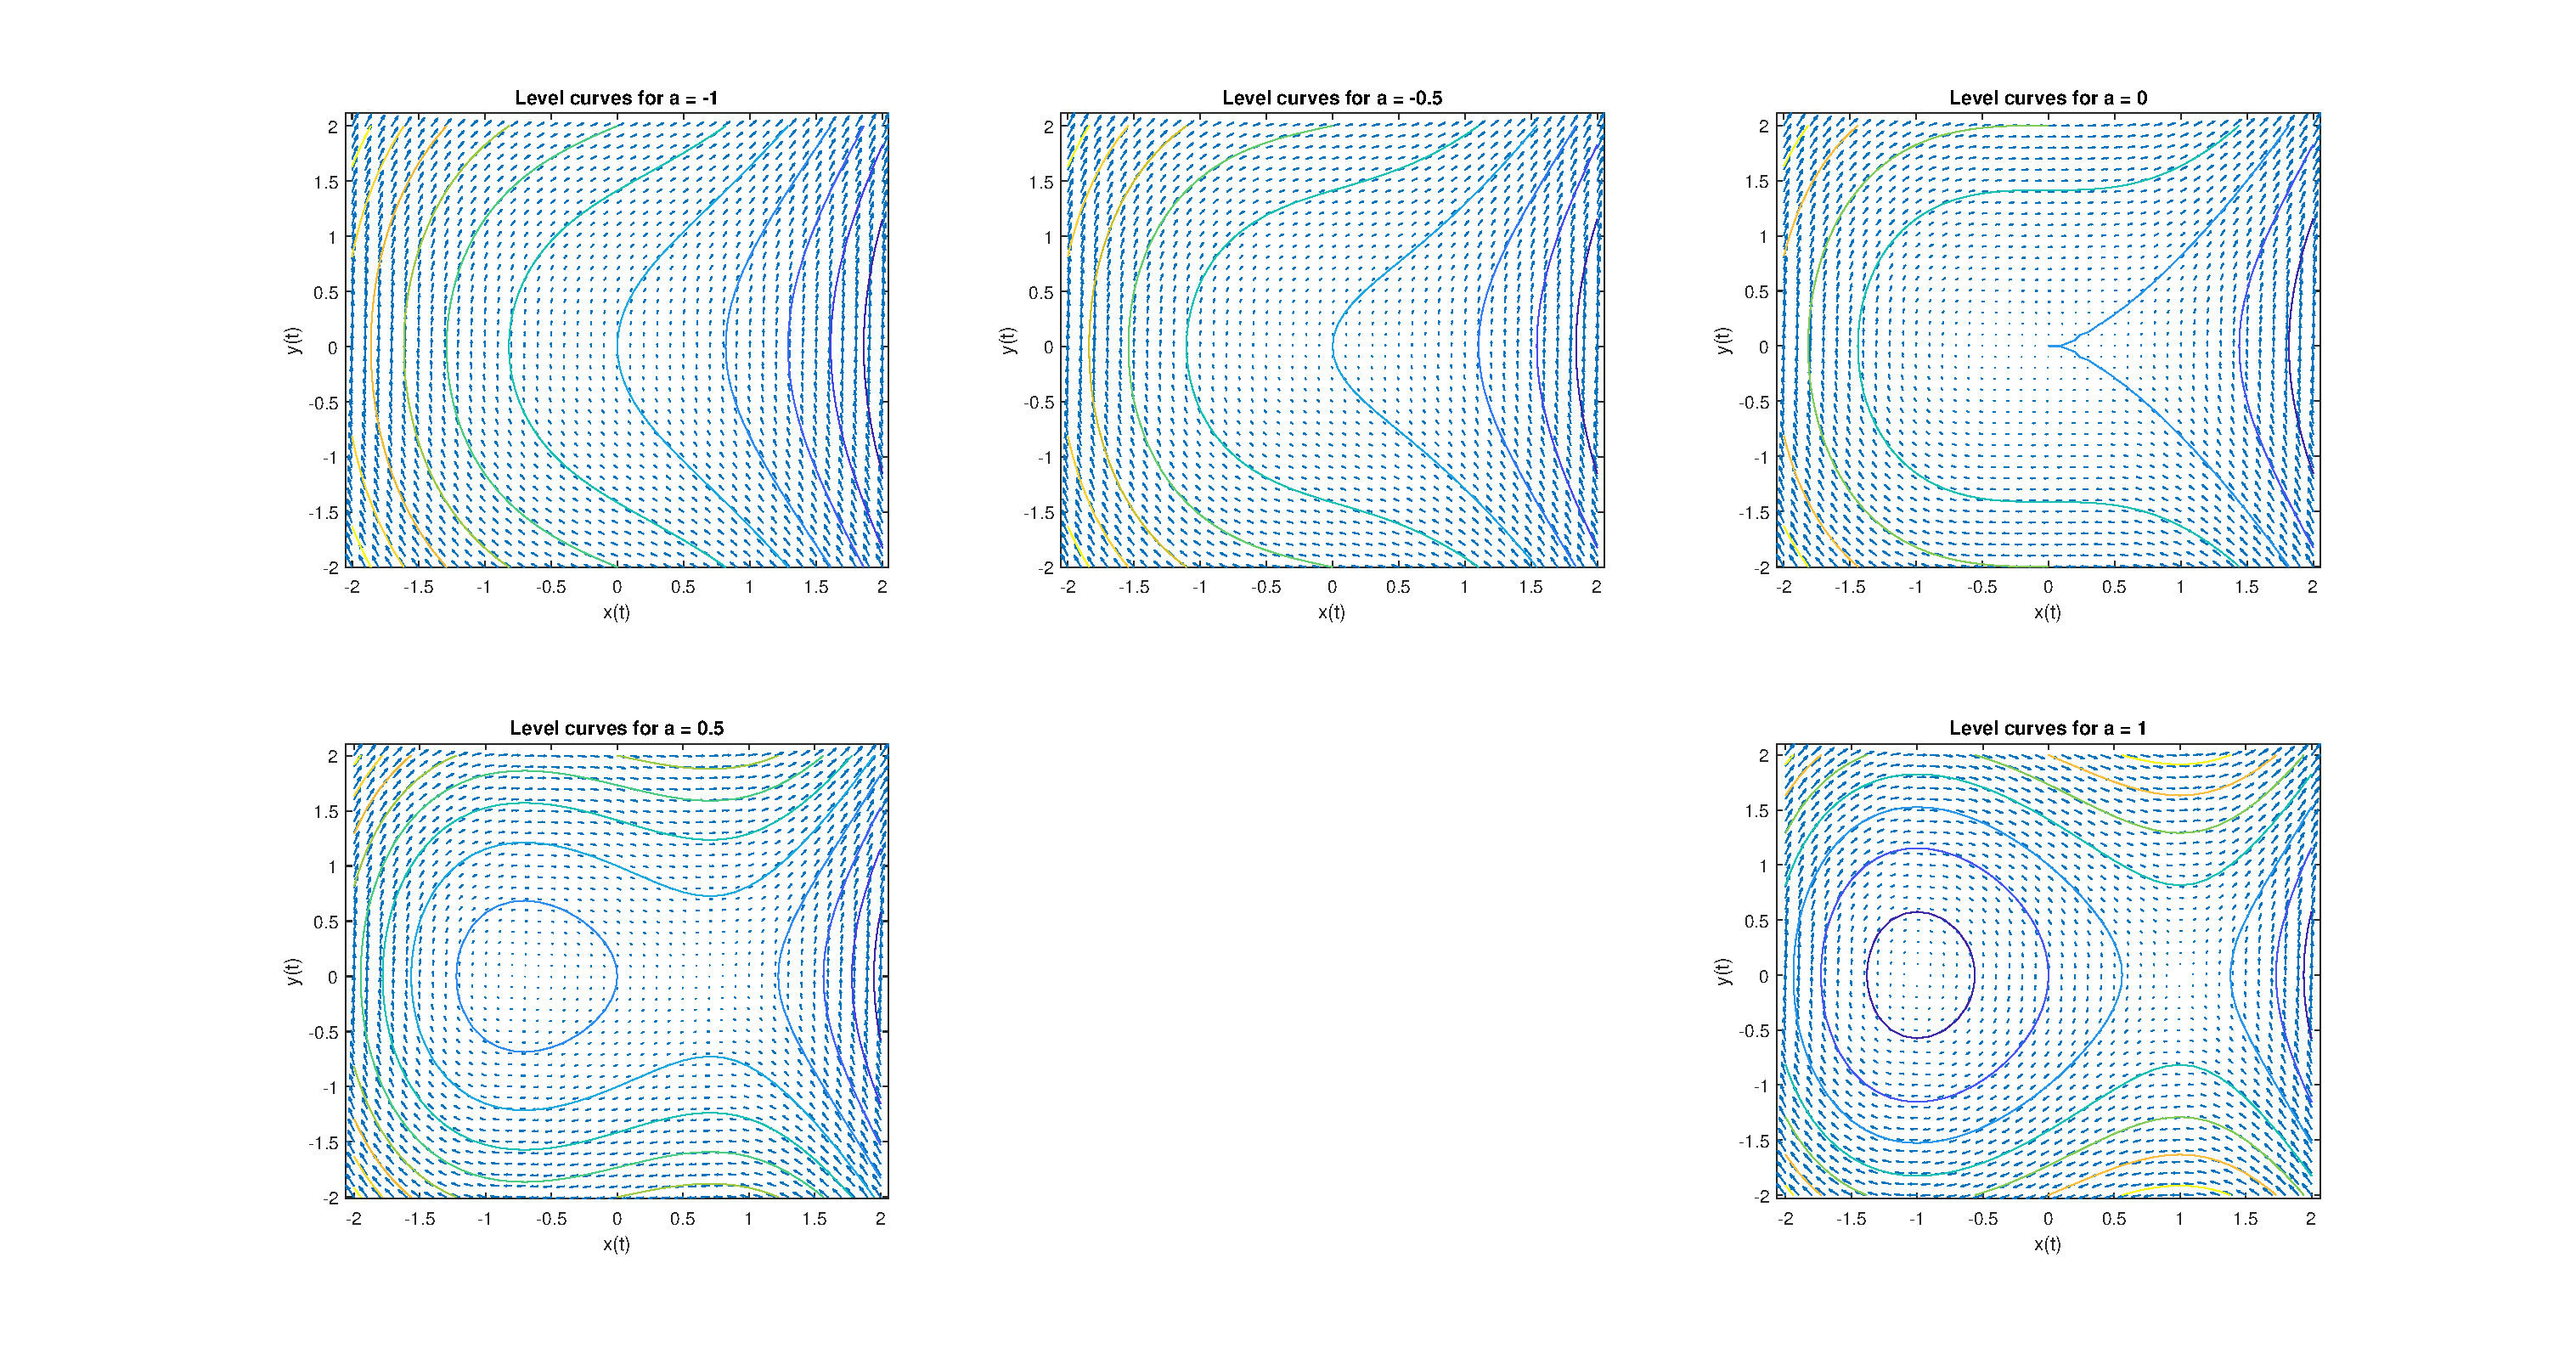
\includegraphics[trim={2in 0 1.5in 0}, width=\linewidth]{Figures/hamiltonian}
	\caption{Phase portrait of $H(x,y)$}
	\label{fig:hamiltonian}
\end{figure}
\end{Example}

\section{Dissipative Systems}
\subsection{Lyapunov functions}
\begin{definition}[Lyapunov functions \cite{diff_eq}]	
A function $L(x(t), y(t)$ is called a \emph{Lyapunov function} for a system of differential equations if, for every solution $(x(t), y(t))$ that is not an equilibrium solution of the system,
\begin{align}
\derivative{}{t} L(x(t), y(t))  \leq 0
\end{align}
for all $t$ with strict inequality except for a discrete set of $t$'s. 
\end{definition}
A Lyapunov function is never increasing along nonequilibrium solutions.

\subsection{Damped Pendulum}
For a pendulum with mass $m = 1$ and length $l = 1$ with a dampening coefficient of $b$, the system describing the motion in polar coordinates is
\begin{align}
\derivative{\theta}{t} &= \omega \\
\derivative{\omega}{t} &= - b \omega - g \sin\theta
\end{align}
where $\theta$ is the angular displacement and $\omega$ is the angular velocity of the pendulum.

The system has steady-states at $(\theta, \omega) = (\pm 2n\pi,0)$ where $n = 0, 1, 2, \ldots$ which correspond to the pendulum being parallel to the vertical and at $((\theta, \omega) = (\pm (2n + 1)\pi,0))$ which corresponds to the pendulum being perpendicular to the vertical. 

Since there is friction involved in the system, the system won't be Hamiltonian and the total energy of the system will be dissipated as time evolves. This can be proven by using the Hamiltonian function for an ideal pendulum from Eq. \ref{eq:hamiltonian_pendulum}. 
\begin{align}
\derivative{}{t}H(\theta(t), \omega(t) &= \frac{\partial H}{\partial \theta} \derivative{\theta}{t} + \frac{\partial H}{\partial \omega} \derivative{\omega}{t} \\
&= (g \sin\theta ) \omega + \omega (- b \omega - g \sin\theta) \nonumber \\
&= - b \omega^2 \\ 
&\leq 0 \nonumber
\end{align}
Since $\derivative{H}{t}$ is always strictly non-positive, but not zero for all solution curves, $H$ is not a Hamiltonian function, but a Lyapunov function. Physically, it means that the pendulum loses energy over time.  

In Figure \ref{fig:damped_pendulum}, the phase plot of a damped pendulum shows the dissipation over time. While the Hamiltonian has a center along the steady-states, the damped pendulum has spiral-sinks, since the Lyapunov function is decreasing when $\omega \neq 0$.  
\begin{figure}[H]
	\centering
	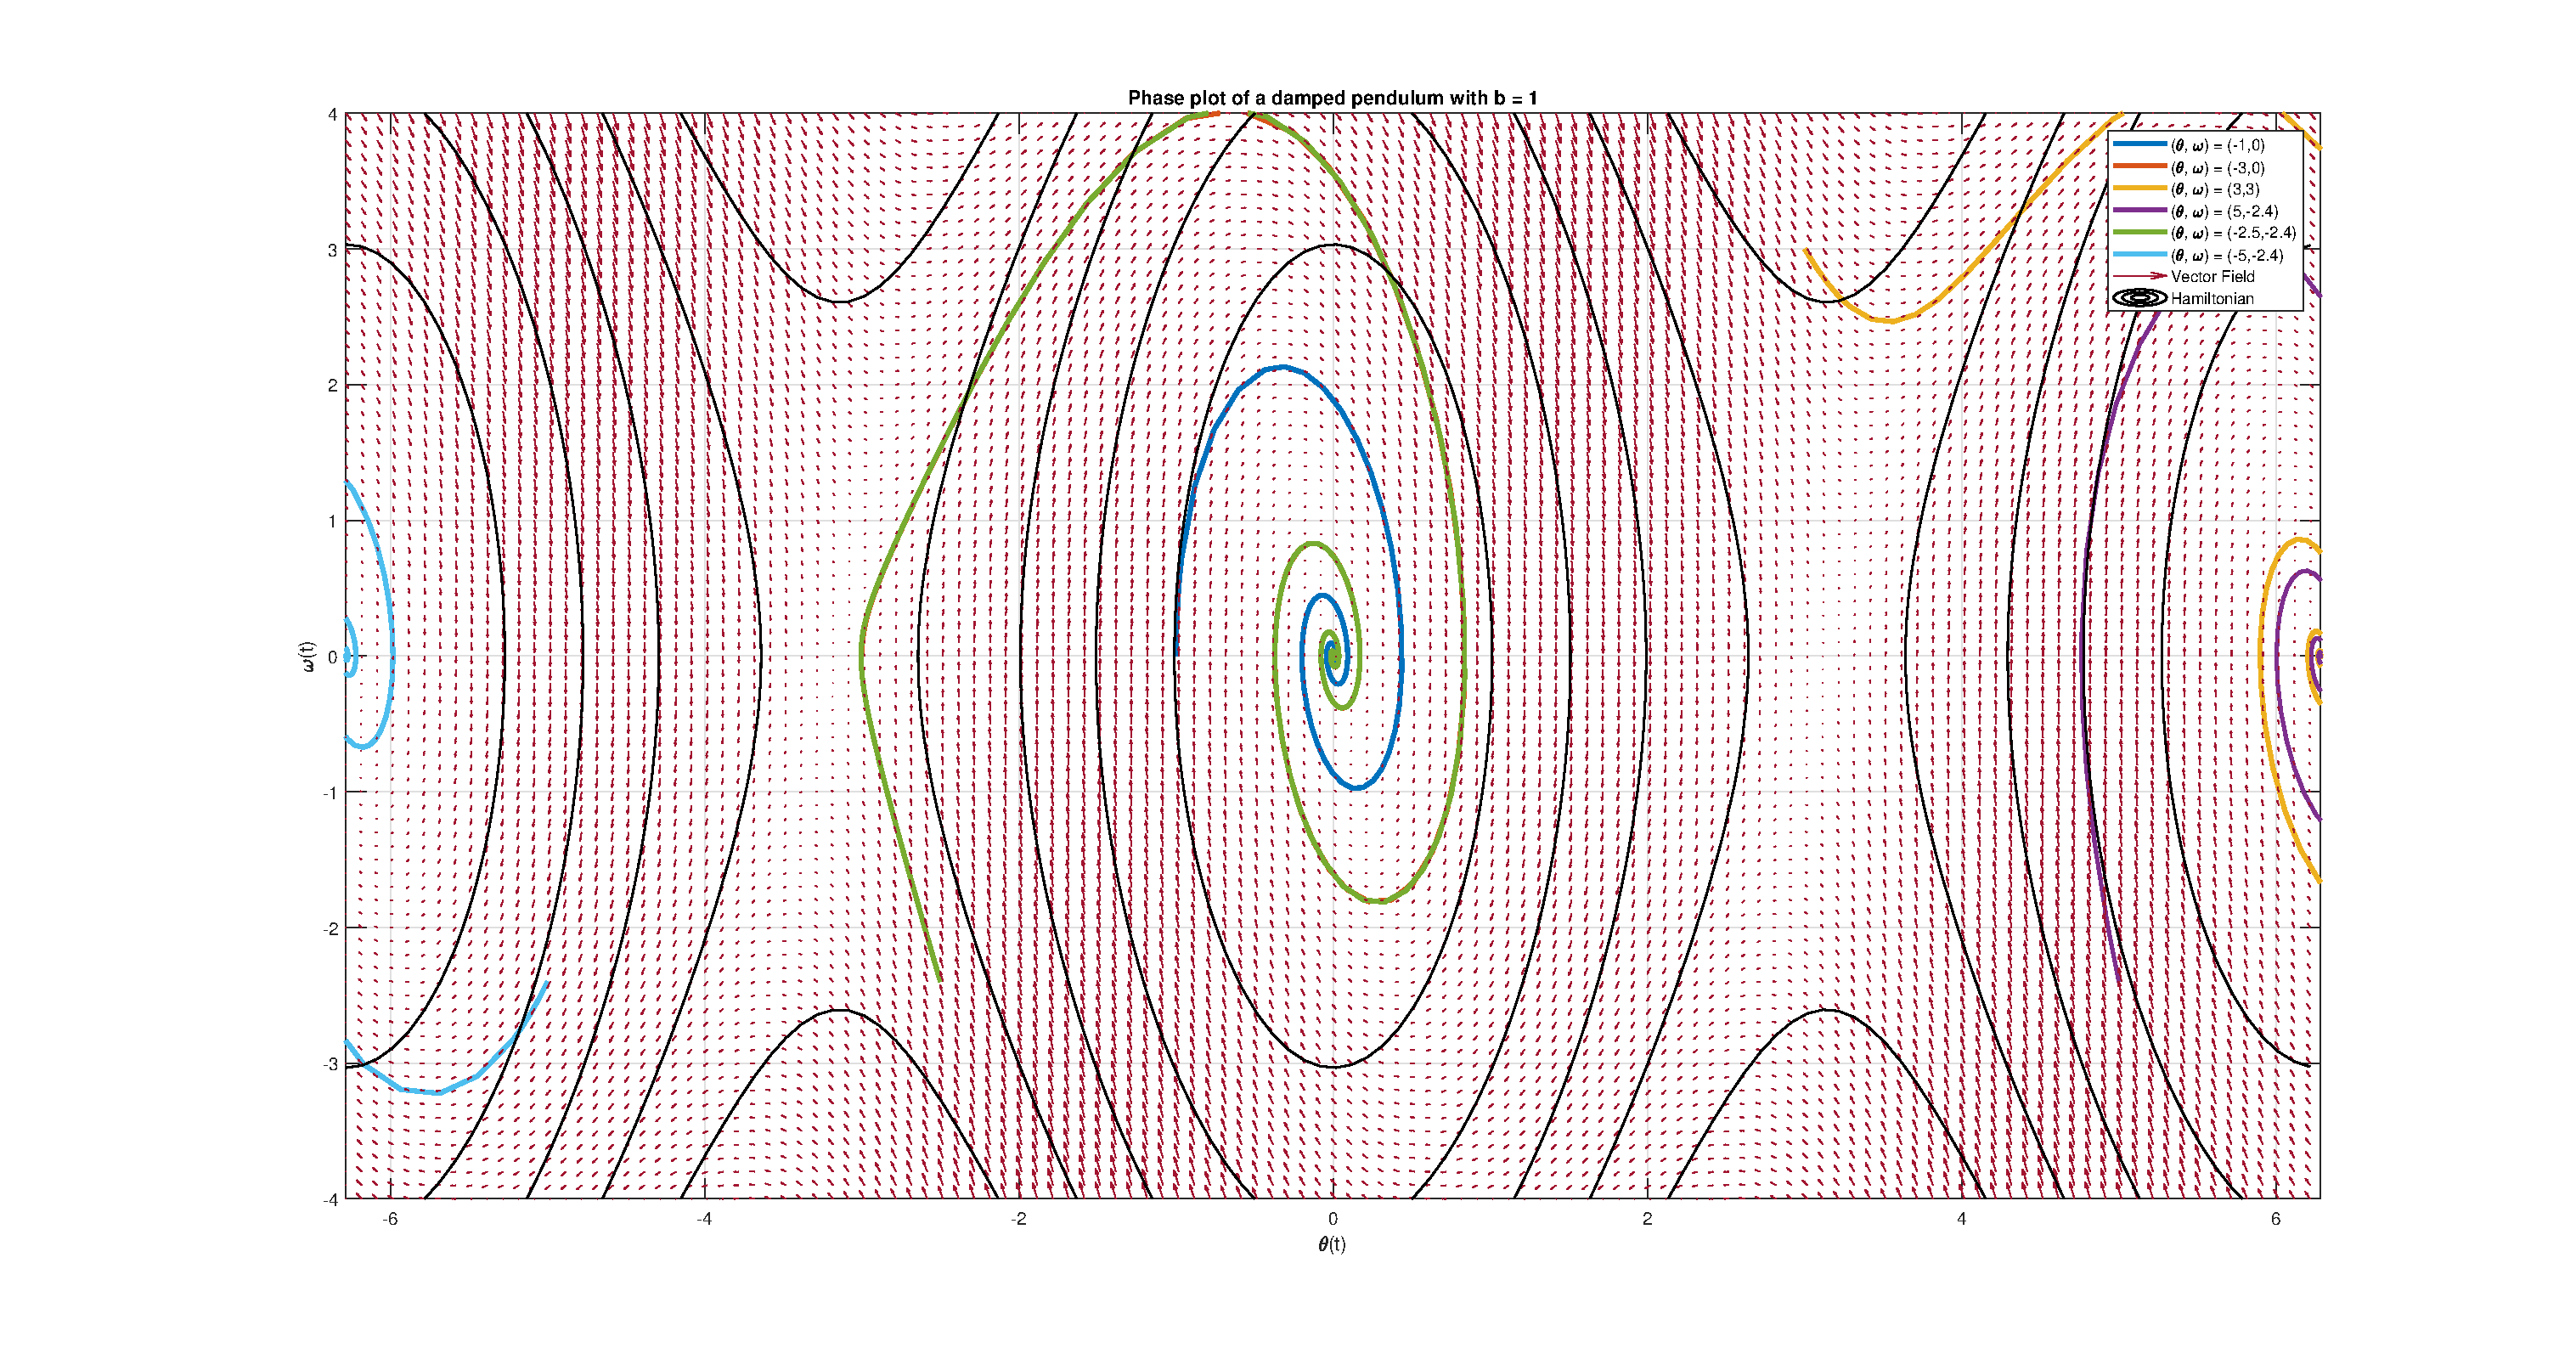
\includegraphics[trim={2in 0 1.5in 0}, width=\linewidth]{Figures/pendulum_phase_damped}
	\caption{Phase portrait of a damped pendulum}
	\label{fig:damped_pendulum}
\end{figure}
\subsection{Examples}
\begin{Example}{1}
	\cite[pp. 528]{diff_eq}
	Given that for a damped pendulum with $l = 9.8$ \si{\meter}, $m = 1$ and $b  =  4$
	The system describing the motion of the system is 
	\begin{align*}
	\derivative{\theta}{t} &= \omega \\
	\derivative{\omega}{t} &= - 4\omega - \sin\theta
	\end{align*}
	The Jacobian of the system is given by 
	\begin{align*}
	J &= \begin{bmatrix}
	0 & 1 \\
	-\cos\theta & -4 
	\end{bmatrix}
	\end{align*}
	Thus, the eigenvalues of the Jacobian at the equilbrium point $(0,0)$ are $\lambda_{1,2} = -2 \pm \sqrt{3}$. Since both the eigenvalues are negative and real, the point $(0,0)$ is a sink. At the point $(\pi, 0)$, the eigenvalues of the Jacobian are $\lambda_{1,2} = -2 \pm \sqrt{5}$. Since the eigenvalues are real and have opposing sides, the point $(\pi,0)$ is a saddle point. As seen in Figure \ref{fig:example_damped_pendulum}, the point $(0,0)$ is a sink and all solutions converge towards that point. The point $(\pi, 0)$ is a saddle point and the solutions diverge away from the point. 
	\begin{figure}[H]
		\centering
		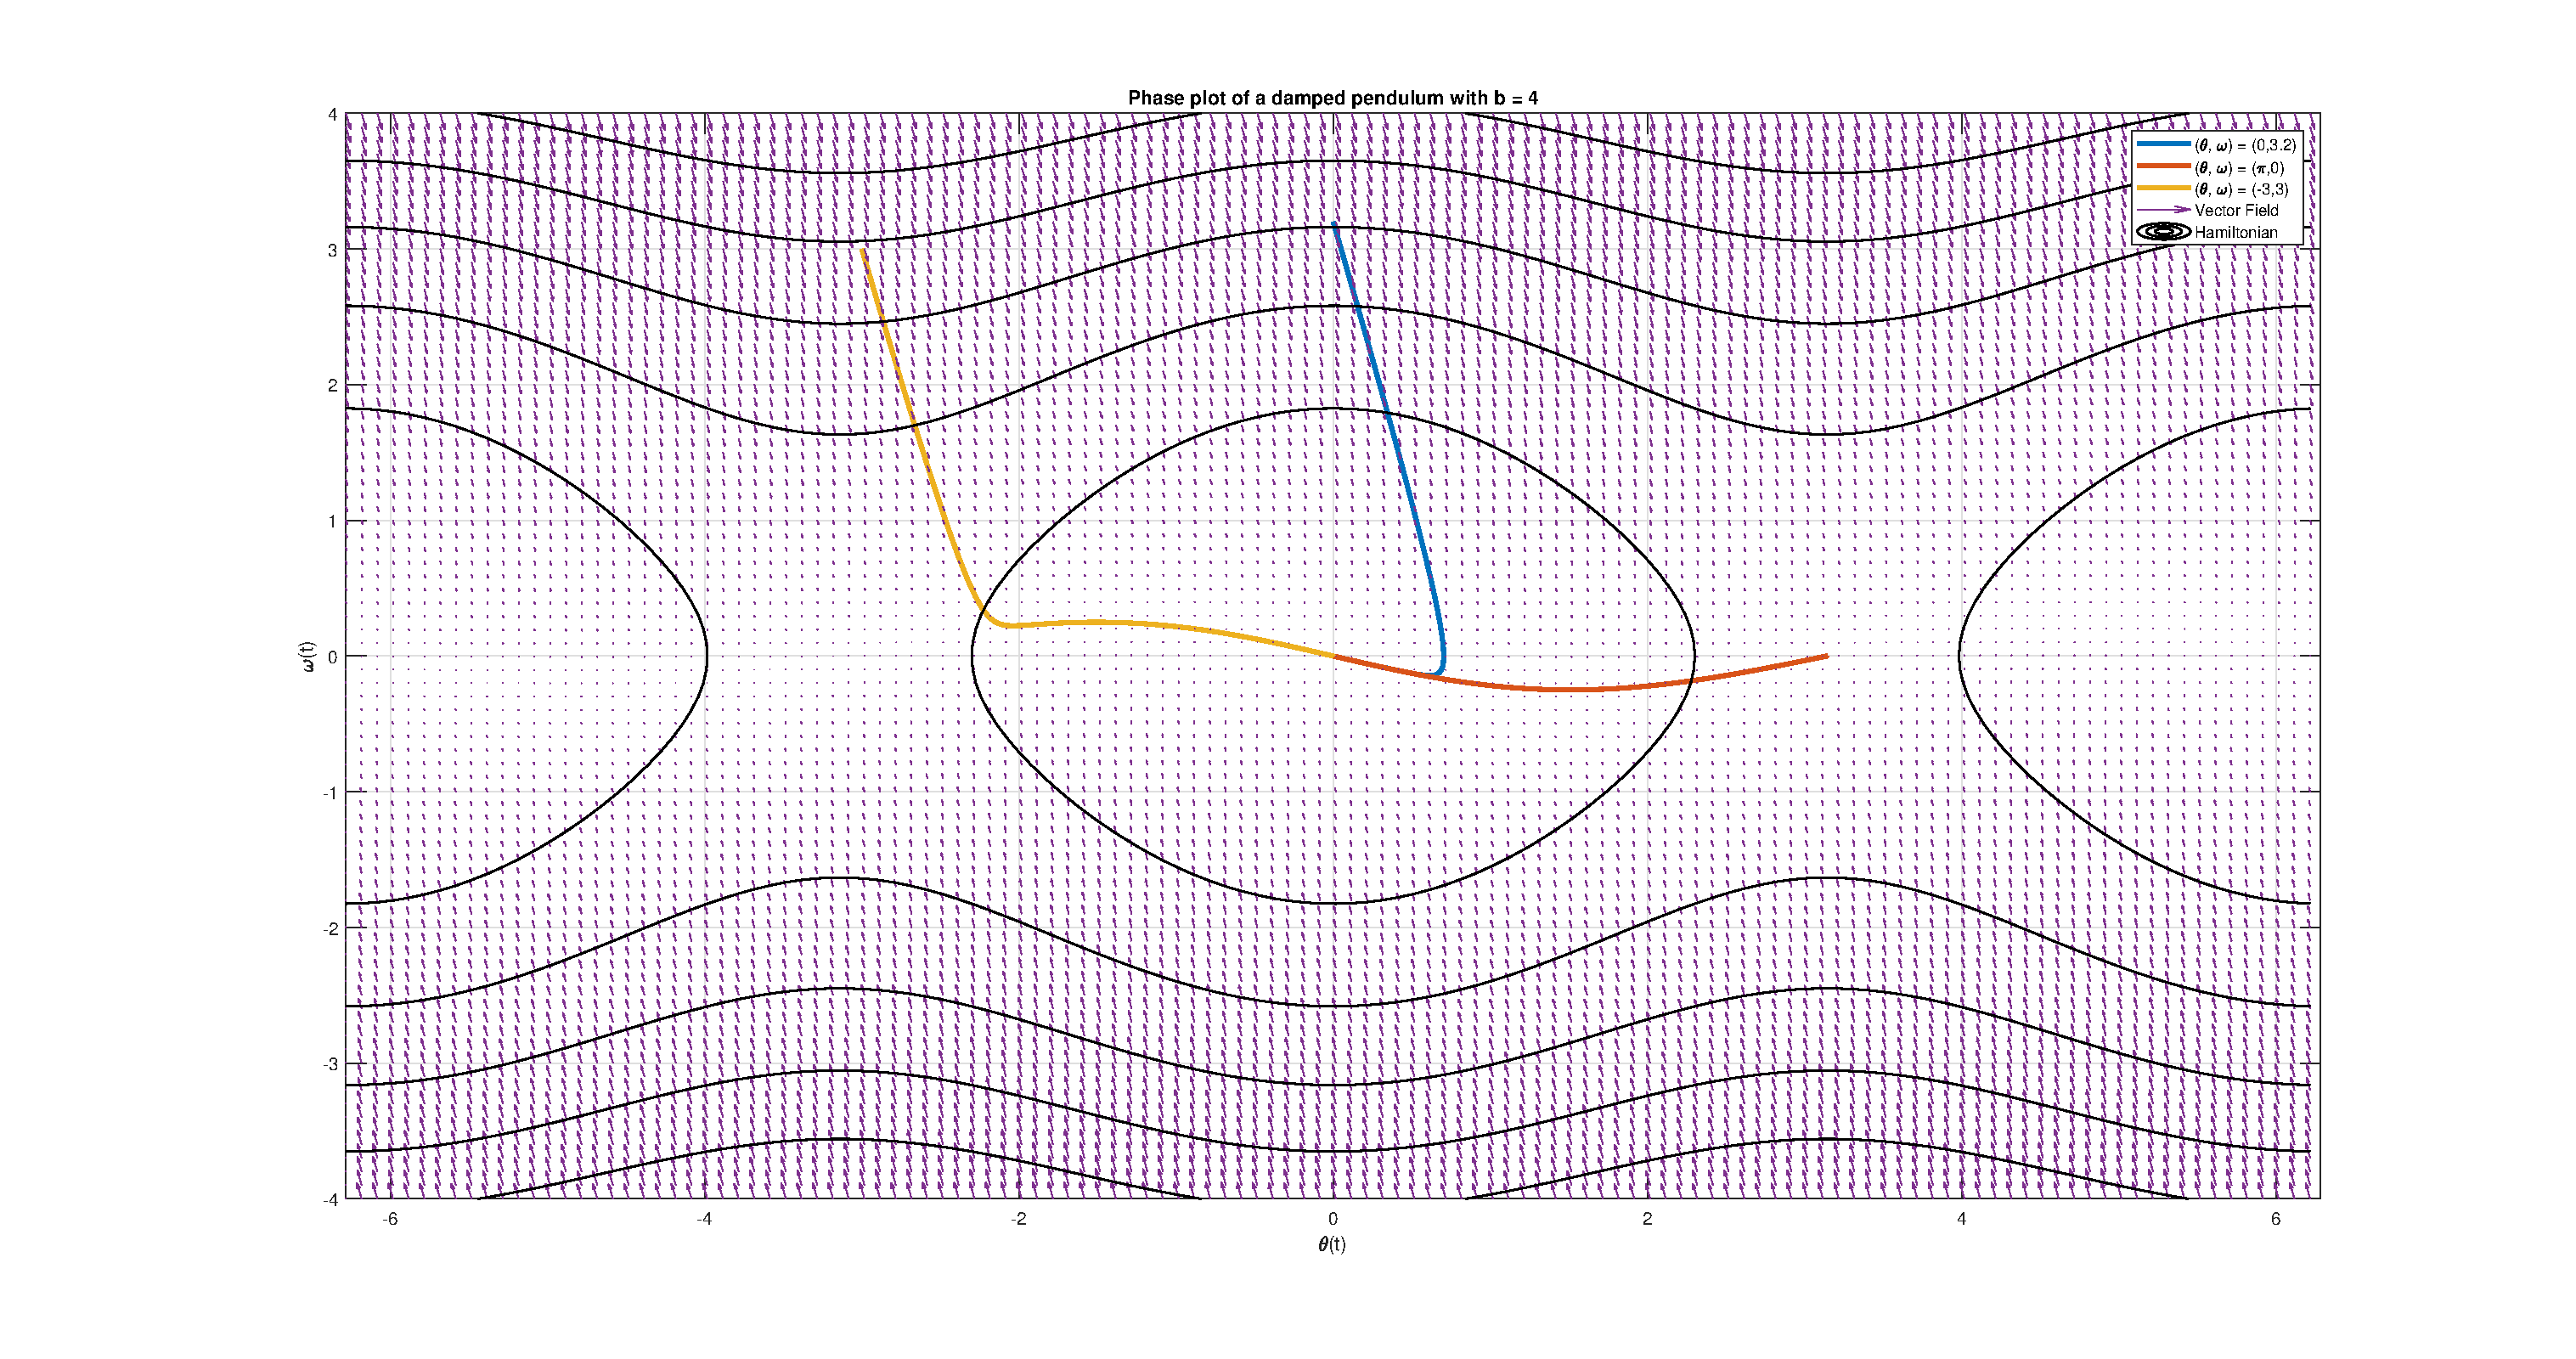
\includegraphics[trim={2in 0 1.5in 0}, width=\linewidth]{Figures/example_damped_pendulum}
		\caption{Phase portrait of a damped pendulum with $m = 1$, $l = g = 9.8$ and $b = 4$}
		\label{fig:example_damped_pendulum}
	\end{figure}
\end{Example}
\section{Appendix}
\lstinputlisting{numerical_soln.m}
\bibliography{citations}
\bibliographystyle{}

\end{document}
